\chapter{Results}
The aim of this research is to determine whether the here proposed S4VD approach is able to find biological relevant and stable biclusters in gene expression data. To this end, we applied the S4VD to a well known lung cancer gene expression data set (Bhattacharyee et al., 2001) \nocite{Bhattacharjee2001}. Furthermore, to examine the influence of increasing levels of noise regarding the performance of the S4VD algorithm, we performed a simulation study. The S4VD algorithm was compared with the SSVD method, the improved Plaid Model (Turner et al., 2005) and the ISA (Bergmann et al., 2003).  The ISA and the Plaid Model are known to be closely related to the SVD.  

\section{Simulation study}
In the first part of the simulations we generated $100$ artificial data matrices comprising $p=1000$ genes and $n=100$ samples, where each entry of the data matrix is set to $0$. In each dataset we randomly assigned $100$ genes and $10$ samples to a bicluster that shows constant upregulated gene expression represented by a value of $1$ in the data matrix. Normally distributed noise $\text{N}(0,\sigma)$ was added to each entry of the data matrix. We examined different noise levels in the range of $\sigma=(0,0.1,\cdots,1)$. In the second part of the simulation study $100$ data matrices of the same dimension were generated. This time four biclusters were included where each consists of $100$ genes and $10$ samples. Constant up- and down-regulation was represented by values of 1,-1,0.5 and -0.5. For both scenarios the performance of the S4VD algorithm was examined in comparison to the original SSVD algorithm, the improved Plaid Model (PM; Turner et al., 2005) and the ISA (Bergmann et al., 2003). Since the SSVD algorithm does not include a stopping criterion, we considered only the first SVD-layer as result in the first scenario and the first four SVD-layers as the biclustering result in the second scenario. The clustering results were validated by application of an external validation index based on the Jaccard coefficient. In addition, the stability of the clustering results was assessed through the average proportion of falsely selected rows and columns. Details on the validation indices, the remaining biclustering algorithms and their relation to the SVD are provided in the supplementary material. 
\subsection{Scenario 1}
The simulation results of the first scenario are shown in Figure 2. For low noise levels up to $\sigma=0.3$ all biclustering algorithms except the SSVD show an almost perfect performance with relevance and recovery scores mostly equal to one and no falsely selected rows and columns. 
For noise levels of $0.1$ to $0.7$ all biclusters proposed by the SSVD algorithm are too large and on average a proportion around $0.015$ of the rows and $0.012$ of the columns are falsely assigned. This results in relevance and recovery scores around $0.8$. In case of larger noise levels the SSVD algorithm often fails to converge and thus the relevance scores and the number falsely assigned rows and columns approach zero. 
For noise levels above $0.3$ the first bicluster detected by the Plaid Model usually consists of a strict subset of those rows and columns that belong to the true artificial bicluster in the data. Thus the performance of the Plaid Model regarding the relevance and the recovery decreases with noise. 
Furthermore, the algorithm starts to fit the noise and proposes a number of further small biclusters. This explains why the relevance score is inferior compared to the recovery score. Most of these small biclusters correspond to parts of the true artificial bicluster and hence the proportions of falsely assigned rows and columns are close to zero. Beginning with a noise level of $0.5$ the ISA proposes an increasing number of biclusters of which only one shows a strong agreement with the true bicluster. Even after applying the additional filtering functions available in the \textit{isa2} R-package (Csardi et al., 2010) some nonsense biclusters remain. Thus both scores start to decrease with noise but are superior to the Plaid Model. The number of falsely assigned rows and columns increases with the noise level indicating that some of the detected biclusters correspond to fitted noise. Regardless of the noise level the S4VD algorithm always detects a single bicluster that agrees with the true bicluster. For noise levels above $0.6$ the proposed bicluster becomes smaller and represents only a part of the true bicluster. Therefore both scores start to decrease with noise but are superior to that of all other biclustering methods considered in the simulation study. Due to the stability selection the S4VD algorithm rarely assigns false rows and columns to the proposed bicluster and does not detect any additional nonsense clusters. Thus the average proportions of falsely assigned rows and columns are almost zero for all noise levels. 

\subsection{Scenario 2}
The results of the second part of the simulation study are shown in Figure 3. For noise levels below $0.3$ the ISA and the S4VD showed relevance and recovery scores around $1$ and the according average proportions of falsely assigned objects are near zero. This indicates that both algorithms are able to correctly detect all of the four artificial biclusters present in the data. 
The Plaid Model algorithm in some cases perfectly revealed the hidden structure, but in other situations depending on the randomly chosen starting values and the noise level the algorithm falsely assigns rows and columns to the biclusters. The stopping criterion of the algorithm depends on a permutation test that can fail to reject unimportant biclusters that correspond to noise. On the other hand for higher noise levels the permutation test also tends to reject biclusters early in the fitting process so that only three or less biclusters are detected. Thus the resulting relevance and recovery scores are highly variable and decrease with noise.
Regarding low noise levels, the SSVD algorithm mostly identifies the correct biclusters but usually falsely assigns some additional rows and columns. This behavior maintains for higher noise levels, but additionally the number of correctly identified biclusters becomes less. 
The performance of the ISA decreases due to an increasing number of identified irrelevant biclusters, starting with noise levels above $0.2$. For noise level $0.5$ the medians of both similarity scores are approximately $0.5$ and the relevance scores show a high variability. For noise levels above $0.5$ the two embedded biclusters generated to have a constant up- and down-regulation of $0.5$ and $-0.5$ are masked by noise, and hence, the ISA as well as the S4VD algorithm tend to miss these clusters. This results in a slight increase of their relevance scores while the recovery scores decrease. Moreover, the relevance scores for both algorithms show a high variability at noise level $0.5$. In summary, the S4VD algorithm outperforms all other biclustering algorithms considered in the simulation study regarding the  similarity scores and the number of falsely assigned rows and columns for all simulation scenarios.

\section{Lung cancer data set}
Three biclusters have been obtained and are shown in the heatmap in Figure 1. The first bicluster corresponds to a subset of $550$ genes and a subset of $28$ samples including $14$ Normal samples and $14$ Carcinoid samples. The second bicluster comprises $12$ Colon samples and one falsely assigned Carcinoid sample together with a subset of $506$ genes. The third bicluster consists of $6$ SmallCell samples and $344$ genes. All other samples and genes have not been assigned to any bicluster. To illustrate that the selected genes represent genes that are associated with the cancer subtypes we performed a geneset enrichment analysis. Tables of all significantly enriched Gene Ontology (GO) terms ($p<0.01$) as well as a description of the analysis can be found in the supplementary material. 
Bhattacharjee et al. (2001) identified several possible marker genes for the different cancer subtypes. A list of eight of these genes together with the corresponding selection probabilities with respect to the three bicluster are shown in Table 1. \textit{TGF-$\beta$ receptor II}, \textit{tetranectin}, \textit{retinoic acid receptor responder 3} and \textit{ficolin 3} are known to be highly expressed in normal lung tissue compared to carcinoid tissue and thus have high selection probabilities for the first bicluster. This coincides with the GO analysis, e.g. two of the $62$ GO-terms that are significantly enriched by the genes corresponding to the first bicluster are \textit{TGF$\beta$ receptor signaling pathway} (GO:0007179) and \textit{response to retinoic acid} (GO:0032526). \textit{Integrin,$\alpha$6} as well as \textit{v-myc} (\textit{c-myc}) are usually overexpressed in colon cancer. These genes have high selection probabilities with respect to the second bicluster. In addition, among the $61$ significantly enriched GO-terms corresponding to the second bicluster is the term \textit{endothelial cell migration} (GO:0043542) which coincides with the fact that the associated samples correspond to colon cancer metastases. The \textit{cell-cycle inhibitor protein p18} and \textit{thymosin-$\beta$} are markers for small cell carcinomas and show high selection probabilities in the third bicluster. Among the $97$ GO-terms significantly enriched in the third bicluster are many cell cycle associated terms, e.g. \textit{cell division} (GO:0051301), \textit{mitotic spindle organization} (GO:0007052) and \textit{cell cycle checkpoint} (GO:0000075). Furthermore, for the first bicluster as well as for the third bicluster the GO-term \textit{positive regulation of Notch signaling pathway} (GO:0045747) is significantly enriched. Alterations of the Notch signaling cascade are known to be associated with several human cancer types. 

\section{Ependymoma data set}
\section{Protein array data set}
%\subsection{Gene Set Enrichment Analysis}

%\newpage

\begin{figure*}[t]
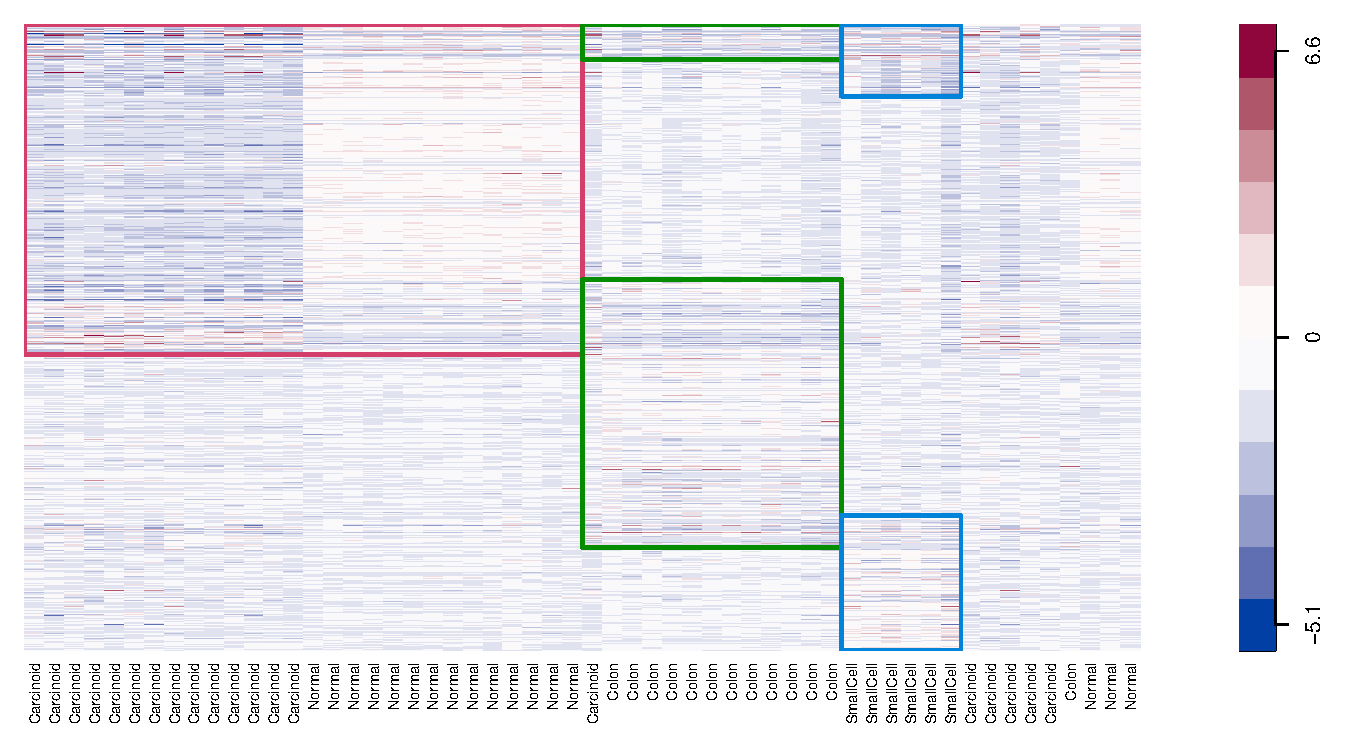
\includegraphics[width=145 mm]{./Bilder/lungheatmap.pdf}
\caption{ Heatmap showing the biclusters identified in the lung cancer data set. Note that the heatmap shows only those genes that have been selected in at least one bicluster. The colored rectangles indicate the genes and samples that correspond to the three biclusters (red corresponds to Bicluster 1, green to Bicluster 2 and blue to Bicluster 3). \label{fig:01} 
}
\end{figure*}

\begin{flushleft}
 \begin{table*}[t]
\caption{Selection probabilities of lung cancer subclass marker genes \label{Tab:01}}
{\begin{tabular}{lrrrr} \hline
Gene & \hspace{4 cm} & Bicluster 1 & Bicluster 2 & Bicluster 3 \\[4pt] 
\hline\\[-4pt]
Retinoic acid receptor responder 3 & & 0.99 & 0.00 & 0.00 \\ 
Transforming growth factor, $\beta$ receptor II (70/80kDa) & & 1.00 & 0.00 & 0.86 \\ 
C-type lectin domain family 3, member B (tetranectin) & & 1.00 & 0.74 & 0.68 \\ 
Ficolin (collagen/fibrinogen domain containing) 3 (Hakata antigen) & &1.00 & 0.71 & 0.98 \\ 
v-myc myelocytomatosis viral oncogene homolog & &0.00 & 1.00 & 0.20 \\ 
Integrin, $\alpha$ 6 & &0.00 & 0.93 & 0.00 \\ 
Cyclin-dependent kinase inhibitor 2C (p18) & &0.00 & 0.00 & 0.91 \\ 
Thymosin $\beta$ & &0.00 & 0.15 & 0.98 \\   
\hline
\end{tabular}}{}%This is a footnote}
\end{table*}
\end{flushleft}

\begin{center}
\begin{figure*}[t]
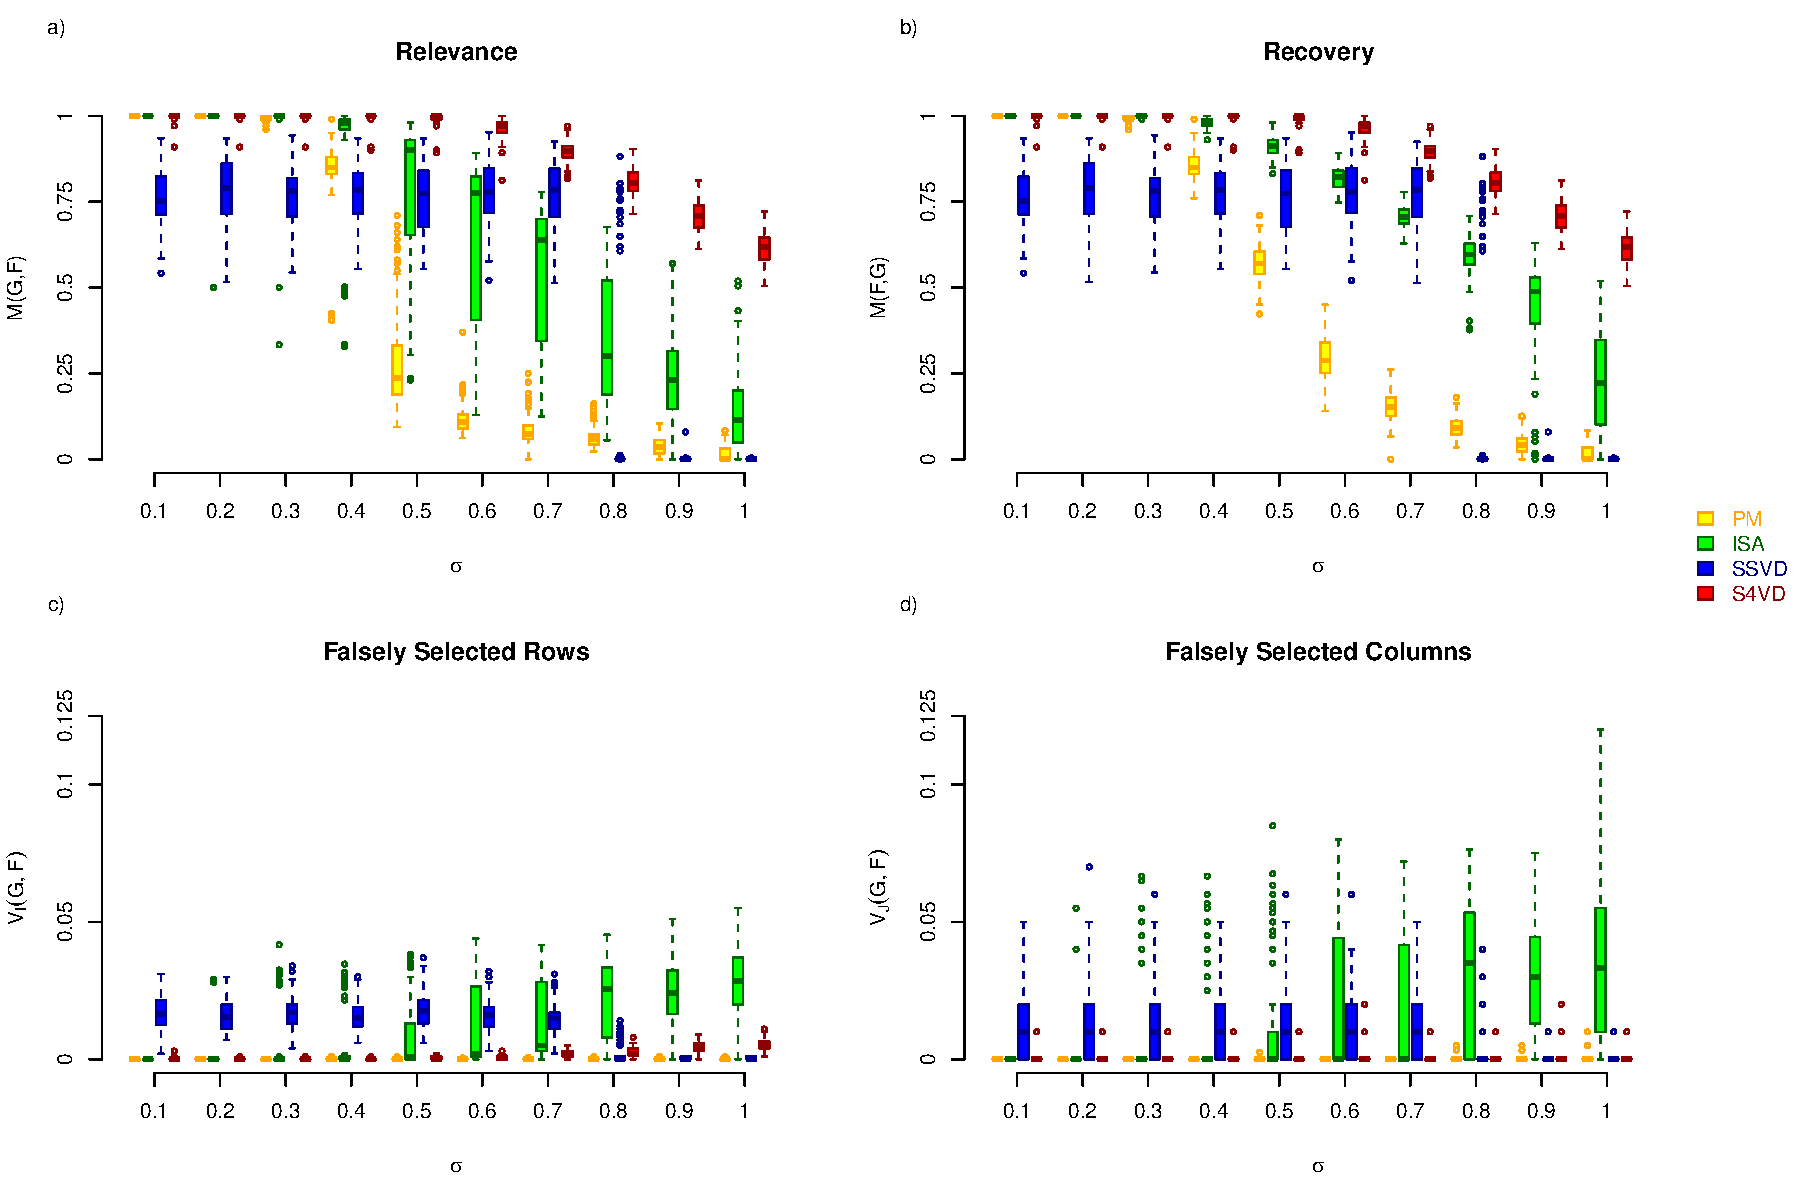
\includegraphics[width=145 mm]{./Bilder/scenario1.pdf}
\caption{ Simulation results of the first scenario. The relevance score $M(G,F)$, recovery score $M(F,G)$ and the average proportions of falsely assigned rows $V_{I}(G,F)$ and columns $V_{J}(G,F)$ are described in the supplementary material. The boxplots show the distribution of these validation indices with respect to the $100$ simulated data sets. $\sigma$ indicates the considered noise level.\label{fig:02} 
}
\end{figure*}
\end{center}

\begin{center}
\begin{figure*}[t]
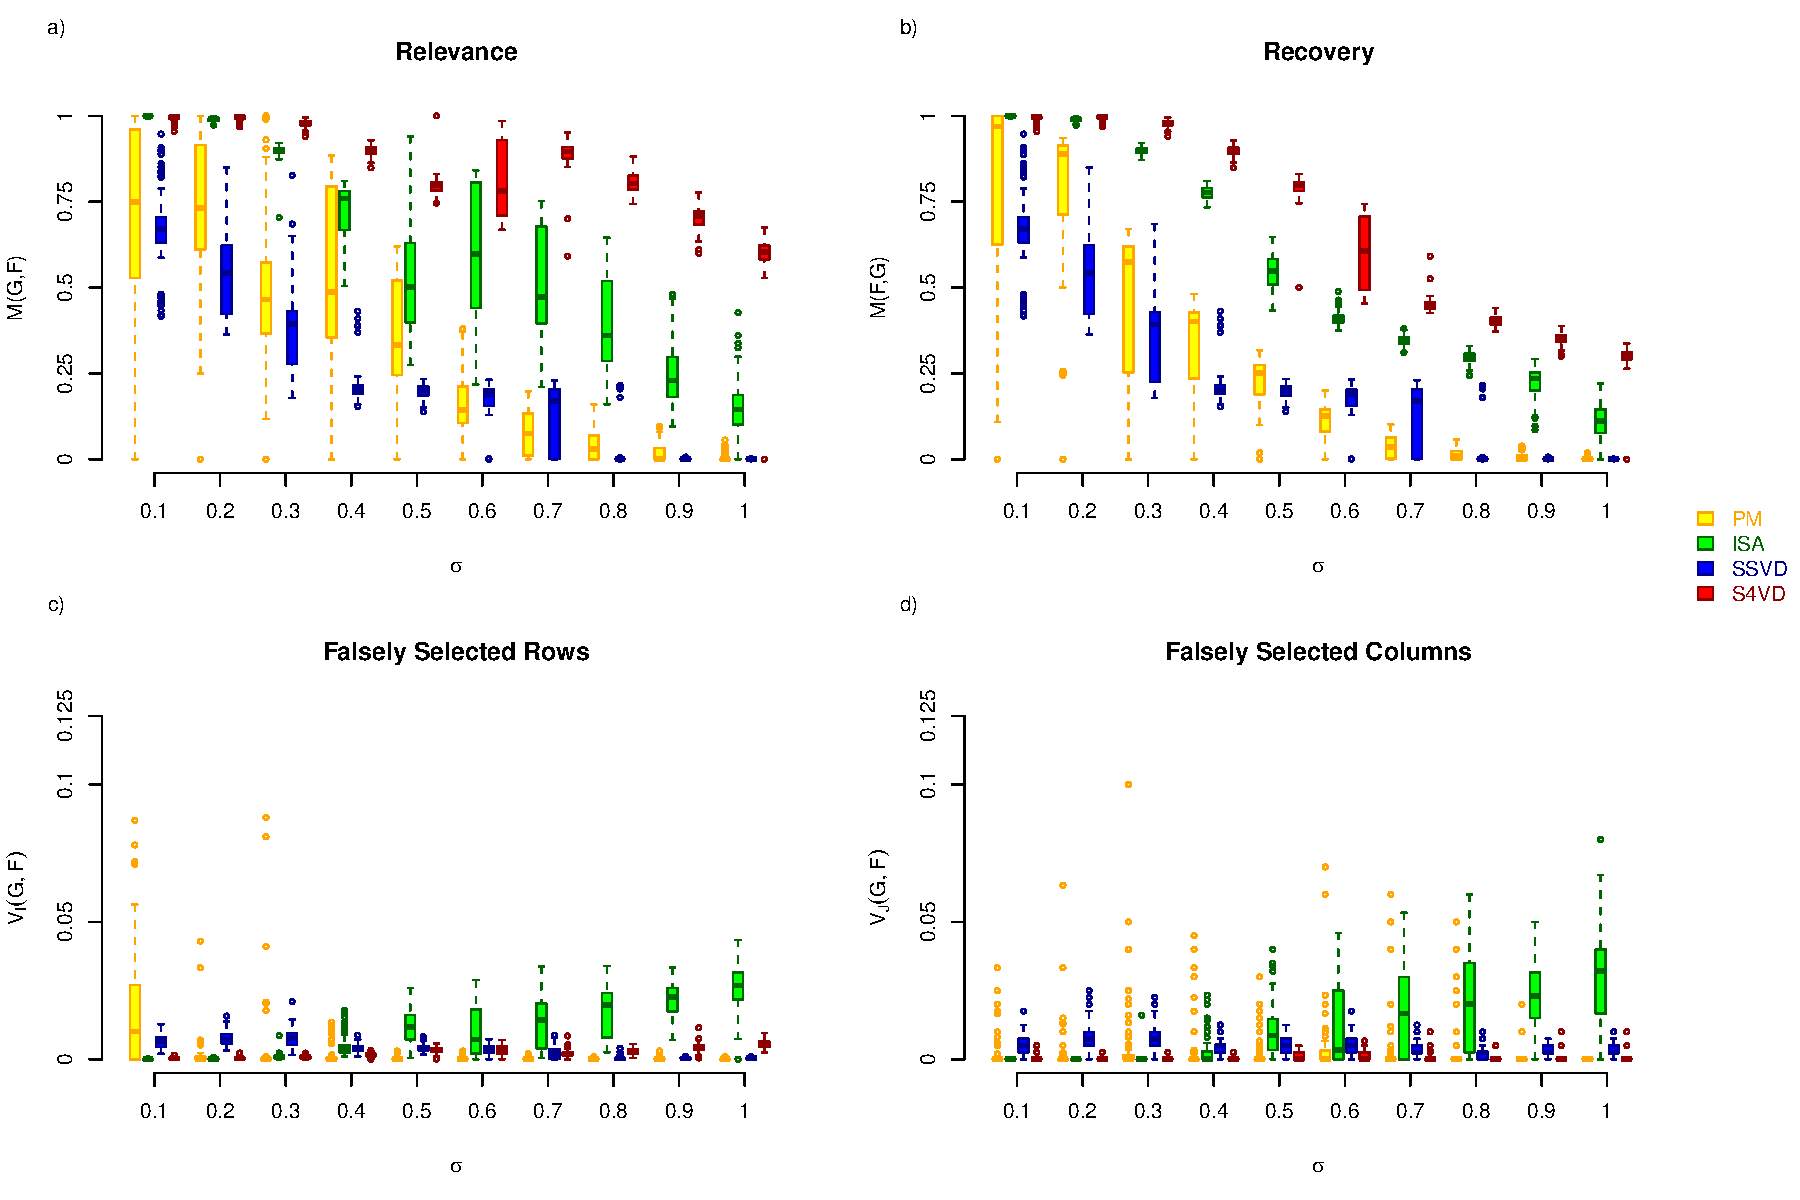
\includegraphics[width=145 mm]{./Bilder/scenario3.pdf}
\caption{ Simulation results of the second scenario. The relevance score $M(G,F)$, recovery score $M(F,G)$ and the average proportions of falsely assigned rows $V_{I}(G,F)$ and columns $V_{J}(G,F)$ are described in the supplementary material. The boxplots show the distribution of these validation indices with respect to the $100$ simulated data sets. $\sigma$ indicates the considered noise level. \label{fig:03} 
}
\end{figure*}
\end{center}

